\section{Forberedelse før test}\label{afs:tests}
Før testene kan gå i gang, skal en testplan udarbejdes således begge versioner bliver testet under samme vilkår med samme funktionaliteter. En tabel over testene kan ses i tabel \ref{tab:resultat_diskret}.
\\

Til test af begge versioner konstrueres en batteriholder til de fire celler som ses på figur \ref{fig:battery_holder}. Her er en ledning forbundet til hver celle for balancering af spændingsmåling.

\begin{figure}[h]
	\centering
	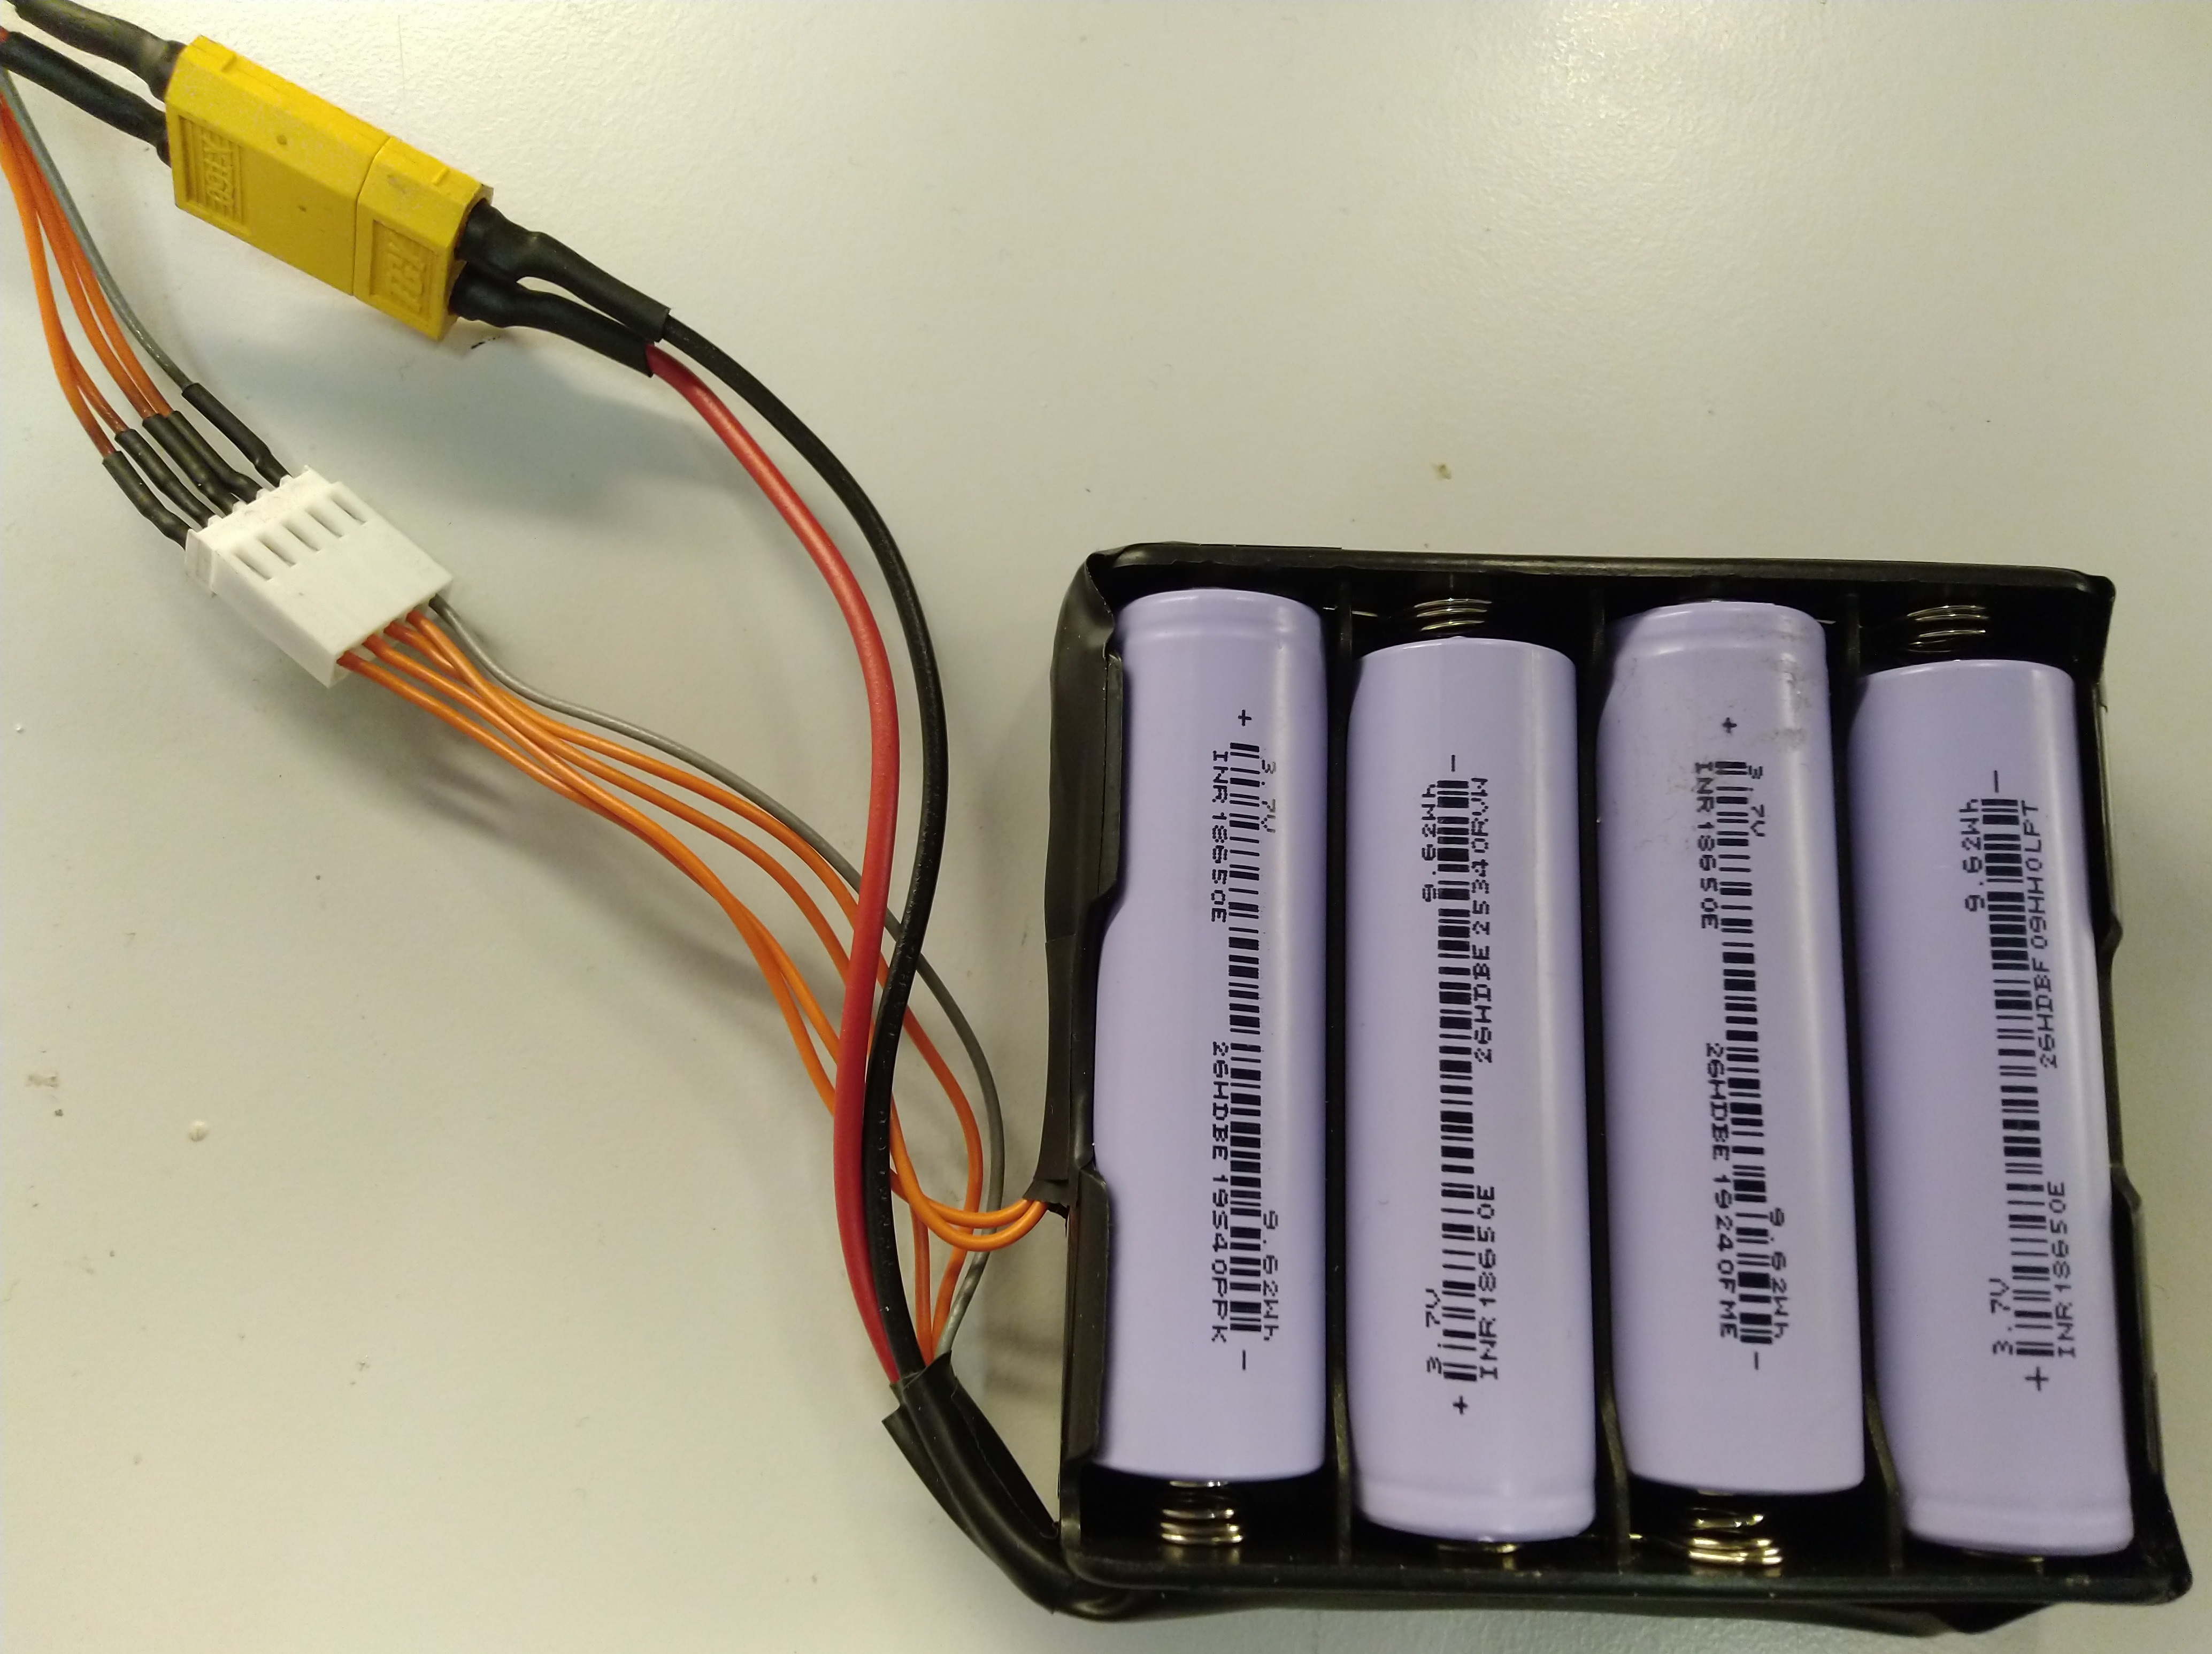
\includegraphics[width=11cm]{billeder/battery_holder.jpg}
	\caption{Batter holder med balanceringsstik.}
	\label{fig:battery_holder}
\end{figure}

\section{Test af IC version}\label{afs:test_ic}
I dette afsnit vil en komplet test opstilling af den integrerede version blive gennemgået og udført.

\subsection{Testopstilling}
Ved brug af en elektrisk belastning vil den maksimale afladestrøm blive testet.



Billede





\subsection{Resultat skema}
Resultaterne fra testene kan ses i tabel \ref{tab:resultat_IC}.


\begin{table}[h!]
	\small
	\centering
	\begin{threeparttable}
		\begin{tabular}{ l l l l l l l }
			\toprule
			\multicolumn{1}{l}{\textbf{Funktionalitet}}          &
			\multicolumn{1}{l}{\textbf{Resultat}}           &
			\multicolumn{1}{l}{\textbf{Kommentar}}   \\ 
			\hline
			Opladestrømsbeskyttelse        & Slår ikke fra  &      \\
			Afladestrømsbeskyttelse        & Slår fra ved $6\ampere$   &      \\
			Balancering af 1 celle         & Virker                    &      \\
			Balancering af 2 celler        & Virker                    &      \\
			Balancering af 3 celler        & Virker                    &      \\
			Balancering færdig             & BMS afbryder              &      \\
			Temperatur - for høj           & BMS afbryder ved   $\SI{45}{\celsius}$       &      \\
			Strømmåling                    & Virker                    &      \\
			Information om kapacitet       & Virker                    &      \\
			Spændingsmålinger              & Virker                    &      \\
			Display                        & Virker ikke               &      \\
			%    &      &       \\
			
			\bottomrule
		\end{tabular}
		%\begin{tablenotes}
		%	\item[a] \textit{Kommentar}
		%\end{tablenotes}
		\caption{Sammenligning af specifikationer.}
		\label{tab:resultat_IC}
	\end{threeparttable}
\end{table} 
\FloatBlock



\section{Test af diskret version}\label{afs:test_diskret}


\subsection{Testopstilling}
Billede

\subsection{Resultat skema}
\begin{table}[h!]
	\small
	\centering
	\begin{threeparttable}
		\begin{tabular}{ l l l l l l l }
			\toprule
			\multicolumn{1}{l}{\textbf{Funktionalitet}}          &
			\multicolumn{1}{l}{\textbf{Resultat}}           &
			\multicolumn{1}{l}{\textbf{Kommentar}}   \\ 
			\hline
			Opladestrømsbeskyttelse        & Slår fra ved $1\ampere$   &      \\
			Afladestrømsbeskyttelse        & Slår fra ved $6\ampere$   &      \\
			Balancering af 1 celle         & Virker                    &      \\
			Balancering af 2 celler        & Virker                    &      \\
			Balancering af 3 celler        & Virker                    &      \\
			Balancering færdig             & BMS afbryder              &      \\
			Temperatur - for høj           & BMS afbryder ved   $\SI{45}{\celsius}$       &      \\
			Strømmåling                    & Virker                    &      \\
			Spændingsmålinger              & Virker                    &      \\
			Display                        & Virker                    &      \\
			%    &      &       \\
			
			\bottomrule
		\end{tabular}
		%\begin{tablenotes}
		%	\item[a] \textit{Kommentar}
		%\end{tablenotes}
		\caption{Sammenligning af specifikationer.}
		\label{tab:resultat_diskret}
	\end{threeparttable}
\end{table} 
\FloatBlock

\section{Delkonklusion}
Ud fra test af begge versioner, kan der konkluderes ....